\documentclass[10pt,letterpaper]{article}
\usepackage{geometry}
\geometry{margin=1in}
\usepackage{graphicx}

\setlength{\parindent}{0pt}
\setlength{\parskip}{0.5em}

%make lists tighter
\usepackage{enumitem}
\setlist{nolistsep}

%reduce spacing before and after section
\usepackage{titlesec}
% reduce section, subsection, etc spacing
\usepackage{titlesec}
\titlespacing*{\section}{0pt}{0\baselineskip}{0\baselineskip}
\titlespacing*{\subsection}{0pt}{0\baselineskip}{0\baselineskip}
\titlespacing*{\subsubsection}{0pt}{0\baselineskip}{0\baselineskip}

%reduce list spacing
\usepackage{enumitem}
\setlist{nosep}

\usepackage[hidelinks]{hyperref}

\title{Lab 3 - Parallelizing $k$-means, Stat 215A, Fall 2026\vspace{-2em}}

% submission must not contain your name
% but feel free to make a version for yourself with your name on it
% \author{Your name}

\begin{document}
\maketitle


\section{Introduction}\label{introduction}

This lab follows the clustering stability approach proposed by Ben-Hur et al. to evaluate the appropriate number of clusters in K-means. K-means requires specifying the number of clusters, $k$, in advance, but determining the appropriate value of $k$ is not always straightforward. One way to address this problem is through clustering stability, which examines whether similar clustering results are obtained from different subsamples of the data. Following Ben-Hur et al., this lab uses binary-coded variables from a linguistic survey dataset and Jaccard similarity to evaluate clustering stability for $k=2$ to $k=10$.

\section{Similarity implementation}

I initially considered three similarity measures: correlation, Jaccard, and matching. However, I ultimately chose Jaccard similarity because it focuses on pairs of observations that are assigned to the same cluster in at least one of the two clustering results. Unlike matching similarity, Jaccard does not count pairs assigned to different clusters in both results as agreements. I thought this would be more appropriate for evaluating whether observations are consistently grouped together across different subsamples.

To calculate Jaccard similarity, I first constructed a contingency table to count the number of observations belonging to each combination of clusters from the two clustering results. I chose this approach because directly comparing every pair of observations would require $O(q^2)$ computations, which could be inefficient for large datasets. Using the contingency table, I calculated the number of observation pairs grouped together in both clustering results and the number grouped together in at least one result. I then divided the former by the latter to obtain Jaccard similarity. This approach avoids creating a large pairwise similarity matrix and reduces the computational complexity to $O(q + k^2)$.

In my initial implementation, I used a Python for-loop to construct the contingency table by counting observations one at a time. When I tested the function with 29,000 randomly generated cluster labels, the average runtime was 5.52 ms. Although this approach avoided the $O(q^2)$ computation, the Python loop still required processing each observation individually, which limited its speed. To improve the implementation, I replaced the for-loop with NumPy's bincount() function, which counts the observations more efficiently. After this modification, the runtime decreased to 1.48 ms for the same input size, making the function approximately 3.7 times faster without changing the Jaccard calculation.

\section{Algorithm 1 implementation}

I used the binary-coded linguistic survey data, consisting of 45,152 observations and 468 binary variables. I evaluated clustering stability for $k=2$ to $k=10$, with 100 repetitions for each value of $k$. I selected the maximum allowed sampling proportion of $m=0.8$ to include as many observations as possible in each subsample. In each repetition, I randomly selected two subsamples without replacement and applied K-means clustering separately to each. I then identified the observations shared by both subsamples and calculated their Jaccard similarity using the function developed in the previous section.

For clustering, I used the KMeans implementation. I kept the remaining parameters, including the initialization method, number of initializations, and maximum iterations, at their default values. Since the primary goal was to evaluate clustering stability across different values of $k$, I did not separately tune these parameters.

To reduce computation time, I used joblib to parallelize the analysis. I treated each combination of $k$ and repetition as an independent task and distributed these tasks across four parallel workers (n\_jobs=4). I used four workers as a practical choice, but I did not systematically compare different numbers of workers to determine the optimal setting.

Although the assignment instructed us to use the SCF cluster, I could not access the server. Therefore, I completed the analysis locally on my Mac mini. The full computation involved 900 similarity calculations and 1,800 K-means fits and took approximately 6 minutes and 33 seconds. I saved the resulting similarity scores in results/S.csv for further analysis.

\section{Result}

{\begin{figure}[htbp]
    \centering
    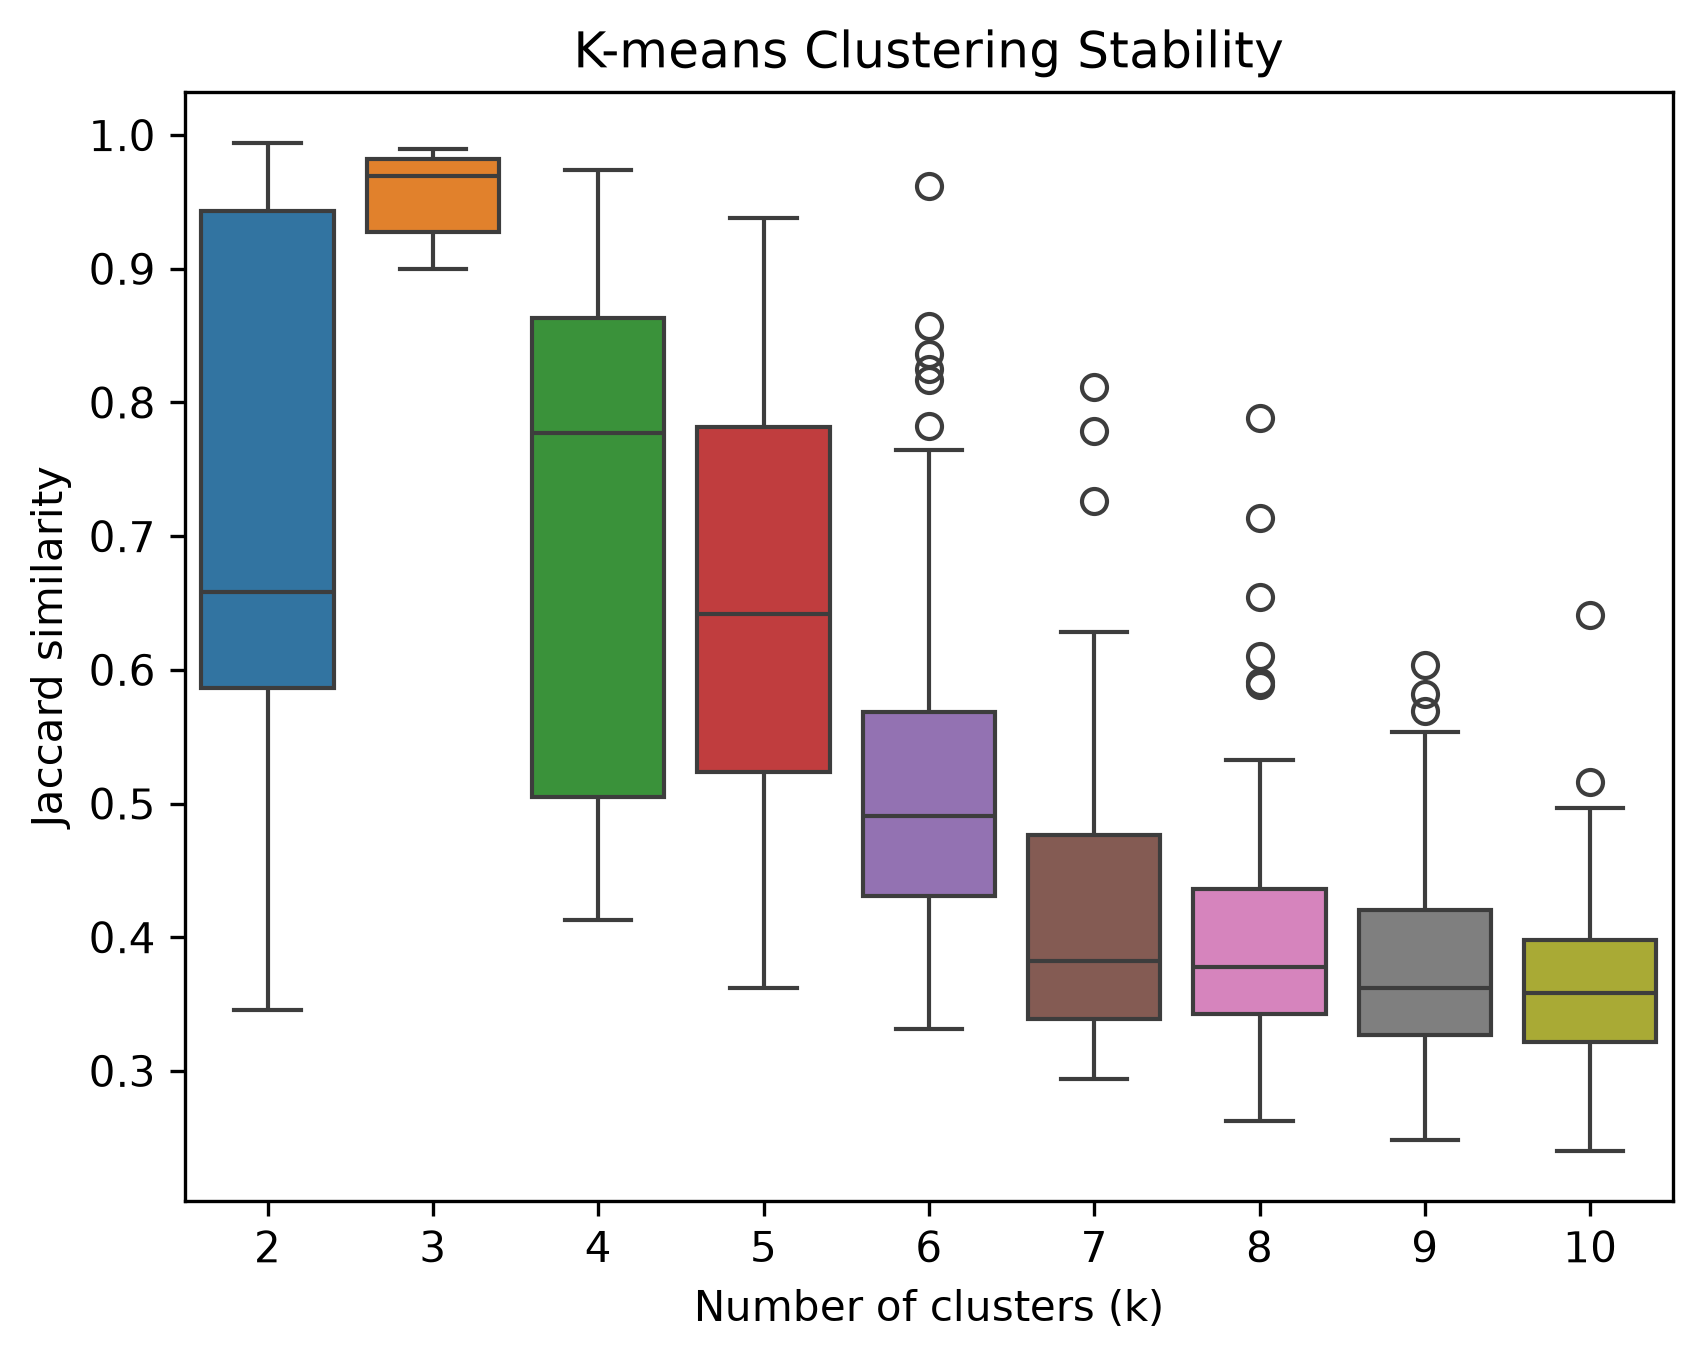
\includegraphics[width=0.85\textwidth]{../figs/stability_plot.png}
    \caption{K-means clustering stability across 100 repetitions using 80\% subsampling.}
    \label{fig:stability}
\end{figure}}

Figure 1 presents the distribution of Jaccard similarity scores across 100 repetitions for each number of clusters from $k=2$ to $k=10$. Among the values tested, $k=3$ showed the highest average Jaccard similarity (0.956) and relatively little variation across repetitions. In contrast, $k=2$ and $k=4$ had lower average similarities of approximately 0.736 and 0.711, respectively, with greater variation. For larger values of $k$, the similarity scores generally decreased, suggesting that the clustering results became less stable as the number of clusters increased.

Based on these results, I would choose $k=3$ because it produced the most consistent clustering assignments across different subsamples. However, high stability does not necessarily mean that the clusters represent meaningful or distinct linguistic groups. In addition, Jaccard similarity can be influenced by the number and sizes of clusters, so directly comparing scores across different values of $k$ has limitations. To further evaluate the appropriate number of clusters, I would compare these results with other methods, such as the elbow method or silhouette scores. 

\section{Academic Honesty}

I certify that I completed this assignment individually and that I have acknowledged any external assistance, including the use of AI tools, as required by the course instructions.

\subsection{LLM Usage}

I utilized ChatGPT to help understand coding and statistical concepts. Specifically, for unfamiliar code, I requested examples to learn how it functions before writing my own code based on those examples. All data processing and analysis were performed independently. Additionally, I used ChatGPT to troubleshoot errors and identify ways to optimize my code.

I spent a significant amount of time understanding the provided examples and applying them myself.
Link: https://chatgpt.com/share/6ad4317b-79f0-83ea-86ca-855c5392540a

\section{Bibliography}

Ben-Hur, A., Elisseeff, A., \& Guyon, I. (2002).
A stability based method for discovering structure in clustered data.
\textit{Pacific Symposium on Biocomputing}, 7, 6--17.
\url{https://doi.org/10.1142/9789812799623_0002}

\end{document}
